% !TEX root = ../main.tex
\subsubsection{Residuals Improvements}
\label{sssec::residuals_improvements}
    To validate the alignment algorithm proposed, it was tested on RG-F data (run $\mathbf{11983}$).
    The improvement in residuals is immediately obvious, as can be seen in figure \ref{fig::res_comparison}, noting the difference in scale between the top and bottom plots.

    \begin{figure}[t!]
        \centering\frame{
        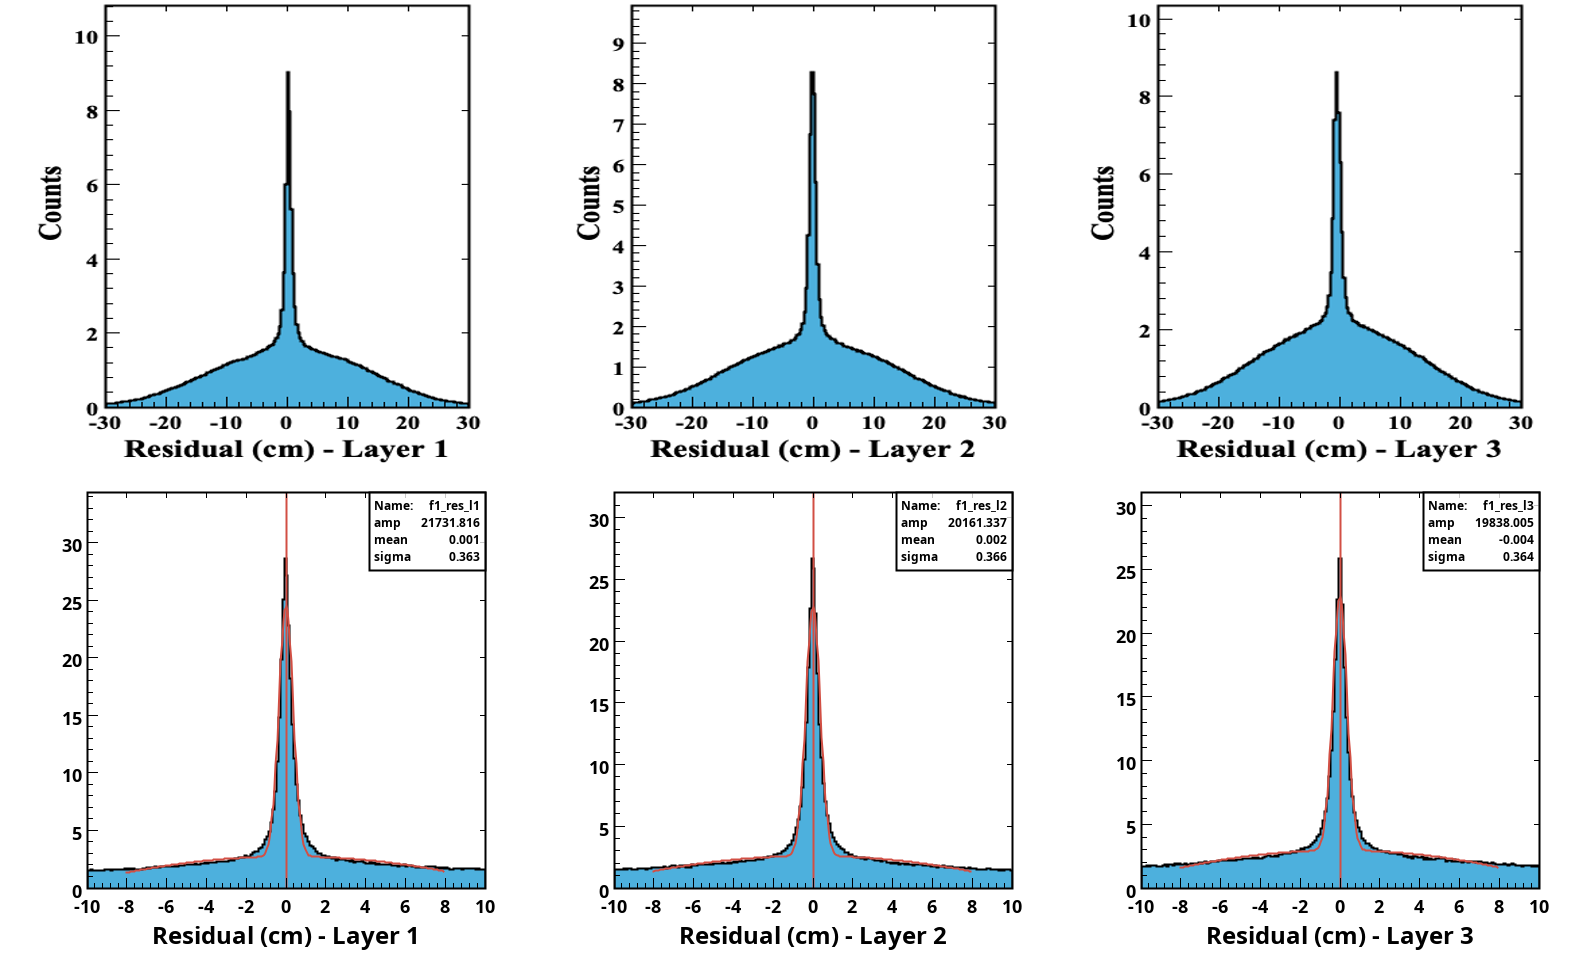
\includegraphics[width=\textwidth]{20res_comparison.png}}
        \caption[Residuals distribution improvement.]{Residuals distribution before (upper image) and after (lower image) alignment.
        Source: \hyperlink{github.com/JeffersonLab/clas12alignment}{CLAS12 alignment software}.}
        \label{fig::res_comparison}
    \end{figure}

    As can be seen in the figure, the $z$ and $\phi$ alignment heavily reduces the background, increasing the number of residuals near the mean of the distribution.
    In addition, the $x$ and $y$ alignment pushes this mean to zero, whereas it was slightly off before.
    Finally, no meaningful results were obtained for pitch and yaw alignment.
    This is attributed to how small the rotations around the $x$ and $y$ axes are, compounded with the fact that three layers do not provide enough data to perform alignment precise enough.

    To measure the mean and $\sigma$ of the distribution, a Gaussian fit was used.
    Its parameters are

     \begin{align*}
        \Big( \text{amp} \cdot \text{gaus}(\mu, \sigma) \Big) &+ \Big( p_0 + p_1\cdot x + p_2\cdot x^2 \Big) \\
        \text{gaussian} \hspace{0.8cm} &+ \hspace{1cm} \text{background}
    \end{align*}

    The results obtained are included in the CCDB at:

    \small\href{clasweb.jlab.org/cgi-bin/ccdb/versions?table=/geometry/fmt/alignment}{\texttt{clasweb.jlab.org/cgi-bin/ccdb/versions?table=/geometry/fmt/alignment}}

    Alignment was also later performed for Run Group M (RG-M) data successfully, proving that the alignment procedure is agnostic to a particular run.
    How this alignment procedure affects the resolution of the entire CLAS12 detector will be explored at the end of the chapter.
